\documentclass{article}
\usepackage[utf8]{inputenc}
\usepackage{amsthm, amsmath, amssymb}
\usepackage[letterpaper,width=150mm,top=20mm,bottom=25mm]{geometry}
\usepackage{textcomp}
\usepackage{xcolor}
\usepackage{soul}
\usepackage{ dsfont }
\usepackage{ mathrsfs }
\usepackage{hyperref}
\usepackage{cancel}
\usepackage{algorithm}
\usepackage{algcompatible}
\usepackage[noend]{algpseudocode}
\usepackage{changepage}%http://ctan.org/pkg/changepage
\usepackage{lipsum}% http://ctan.org/pkg/lipsum
\usepackage{graphicx}
\usepackage{tikz}
\usepackage{lscape}
\usetikzlibrary{shapes.misc, positioning}
\usetikzlibrary{arrows.meta}
\tikzset{>={Latex[width=2mm,length=2mm]}}

\title{Control Flow Graphs so i don't mess up the big document}
\begin{document}
\maketitle

\begin{figure}[h]
    \centering
    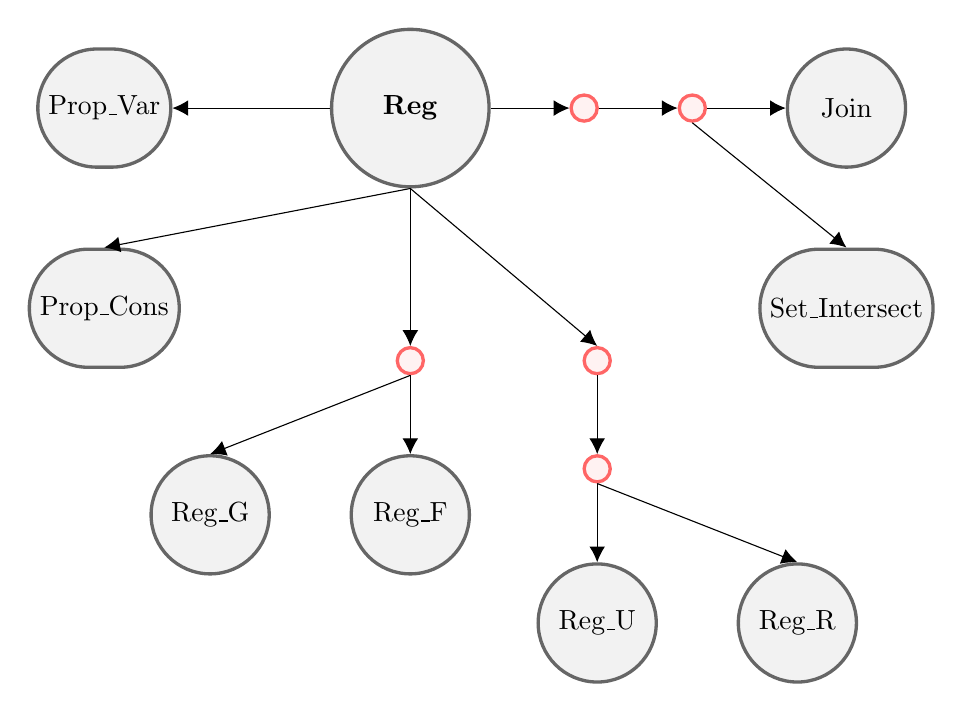
\begin{tikzpicture}[node/.style={rounded rectangle, draw=black!60, fill=black!5, very thick, minimum size=15mm}, bignode/.style={rounded rectangle, draw=black!60, fill=black!5, very thick, minimum size=20mm}, star/.style={circle, draw=red!60, fill=red!5, very thick, minimum size=1mm}]
    
    %Nodes
    \node[bignode](reg){\textbf{Reg}};
    \node[node](prop_var)[left=2 cm of reg]{Prop\_Var};
    \node[node](prop_cons)[below=of prop_var]{Prop\_Cons};
    \node[star](unary_star)[below=2 cm of reg]{};
    \node[node](reg_f)[below=of unary_star]{Reg\_F};
    \node[node](reg_g)[left= of reg_f]{Reg\_G};
    \node[star](temp_binary_star1)[right=2 cm of unary_star]{};
    \node[star](temp_binary_star2)[below= of temp_binary_star1]{};
    \node[node](reg_u)[below=of temp_binary_star2]{Reg\_U};
    \node[node](reg_r)[right=of reg_u]{Reg\_R};
    \node[star](prop_binary_star1)[right= of reg]{};
    \node[star](prop_binary_star2)[right= of prop_binary_star1]{};
    \node[node](join)[right=of prop_binary_star2]{Join};
    \node[node](set_intersect)[below=of join]{Set\_Intersect};
    
    %Lines
    \draw[->] (reg.west) -- (prop_var.east);
    \draw[->] (reg.south) -- (prop_cons.north);
    \draw[->] (reg.south) -- (unary_star.north);
    \draw[->] (unary_star.south) -- (reg_f.north);
    \draw[->] (unary_star.south) -- (reg_g.north);
    \draw[->] (reg.south) -- (temp_binary_star1.north);
    \draw[->] (reg.east) -- (prop_binary_star1.west);
    \draw[->] (temp_binary_star1.south) -- (temp_binary_star2.north);
    \draw[->] (temp_binary_star2.south) -- (reg_r.north);
    \draw[->] (temp_binary_star2.south) -- (reg_u.north);
    \draw[->] (prop_binary_star1.east) -- (prop_binary_star2.west);
    \draw[->] (prop_binary_star2.east) -- (join.west);
    \draw[->] (prop_binary_star2.south) -- (set_intersect.north);
    \end{tikzpicture}
    
    
    
    \caption{Abstracted Graph}
    \label{fig:abstracted graph}
\end{figure}

\begin{figure}[h]
    \centering
    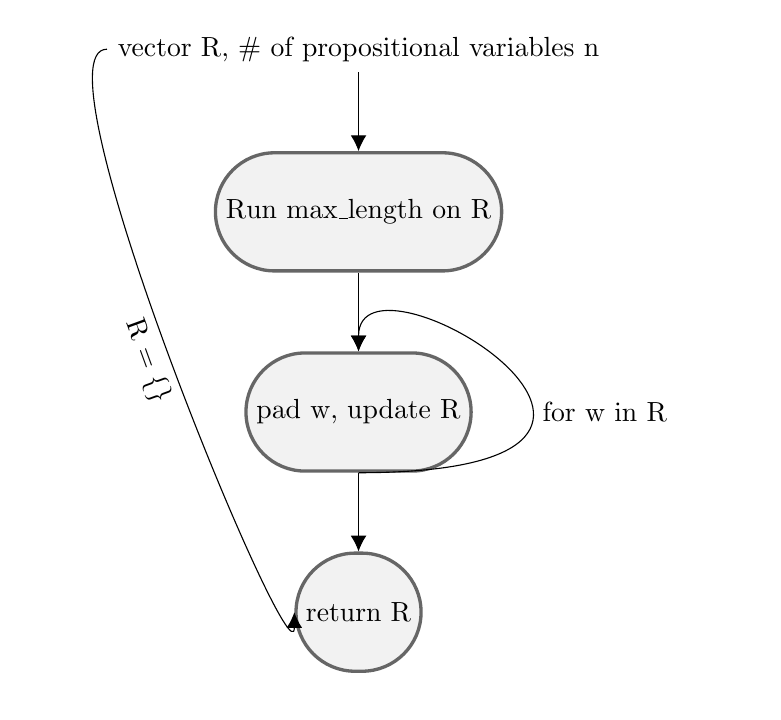
\begin{tikzpicture}[node/.style={rounded rectangle, draw=black!60, fill=black!5, very thick, minimum size=15mm}, bignode/.style={rounded rectangle, draw=black!60, fill=black!5, very thick, minimum size=20mm}, emptynode/.style={draw=none, fill=none, very thick, minimum size=1mm}]
    
    %Nodes
    \node[emptynode](inputs){vector R, \# of propositional variables n};
    \node[node](length)[below=of inputs]{Run max\_length on R};
    \node[node](body)[below=of length]{pad w, update R};
    \node[emptynode](empty_vector)[rotate=-70, left=1cm of body]{R $=\{\}$};
    \node[emptynode](for_loop)[right=.75cm of body]{for w in R};
    \node[node](return)[below=of body]{return R};
    
    %Lines
    \draw[->] (inputs.south) -- (length.north);
    \draw[->] (length.south) -- (body.north);
    \draw[->] (body.south) -- (return.north);
    \draw[->] (inputs.west) .. controls +(left:1 cm) and +(down:1 cm) .. (return.west);
    \draw[->] (body.south) .. controls +(right:5 cm) and +(up:1.5 cm) .. (body.north);
    
    \end{tikzpicture}
    
    \caption{Pad Function}
    \label{fig:pad graph}
\end{figure}

\begin{figure}[h]
    \centering
    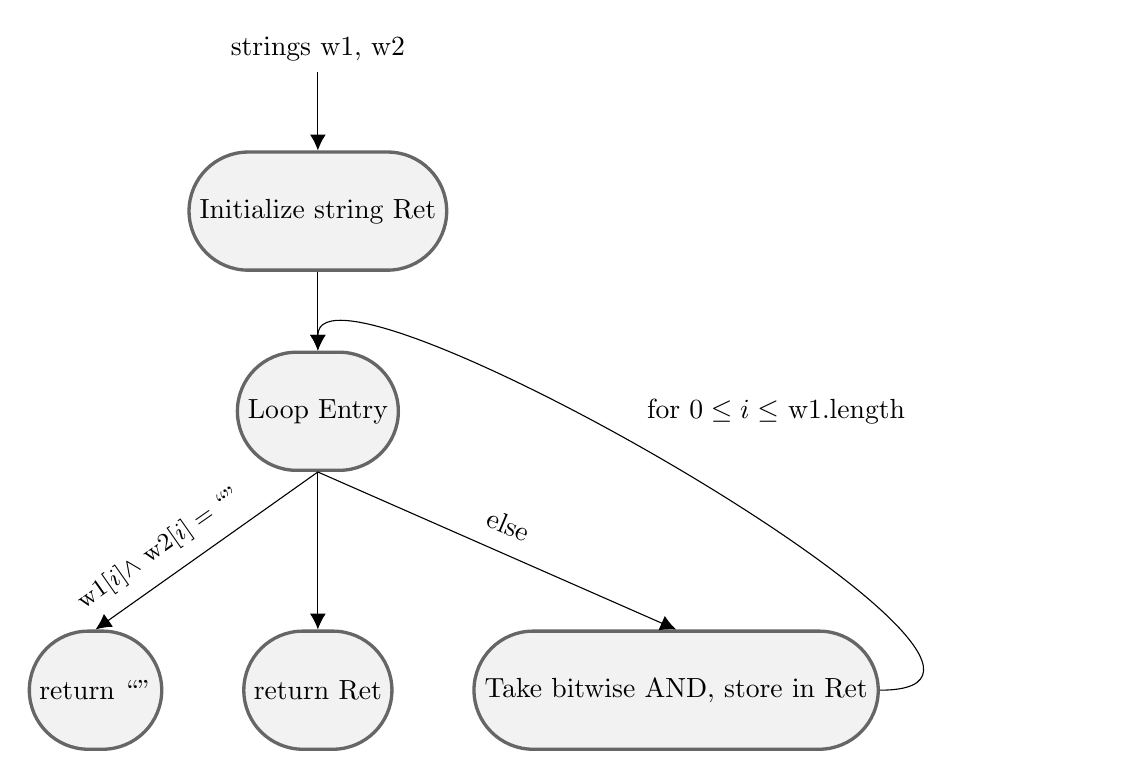
\begin{tikzpicture}[node/.style={rounded rectangle, draw=black!60, fill=black!5, very thick, minimum size=15mm}, bignode/.style={rounded rectangle, draw=black!60, fill=black!5, very thick, minimum size=20mm}, emptynode/.style={draw=none, fill=none, very thick, minimum size=1mm}]
    
    %Nodes
    \node[emptynode](inputs){strings w1, w2};
    \node[node](initialize)[below=of inputs]{Initialize string Ret};
    \node[node](loop_entry)[below=of initialize]{Loop Entry};
    \node[node](return)[below=2cm of loop_entry]{return Ret};
    \node[node](empty)[left=of return]{return ``"};
    \node[node](update)[right=of return]{Take bitwise AND, store in Ret};
    \node[emptynode](placeholder)[below=0.05cm of loop_entry]{};
    \node[emptynode](emptytext)[rotate=35, left=.75cm of placeholder]{\small{w1$[i] \land$ w2$[i] = ``"$}};
    \node[emptynode](placeholder2)[below=0.05cm of placeholder]{};
    \node[emptynode](else)[rotate=-23, right=1.9cm of placeholder2]{else};
    \node[emptynode](updatetext)[right=3cm of loop_entry]{for $0 \leq i \leq$ w1.length};
    
    %Lines
    \draw[->] (inputs.south) -- (initialize.north);
    \draw[->] (initialize.south) -- (loop_entry.north);
    \draw[->] (loop_entry.south) -- (return.north);
    \draw[->] (loop_entry.south) -- (empty.north);
    \draw[->] (loop_entry.south) -- (update.north);
    \draw[->] (update.east) .. controls +(right:3 cm) and +(up:1.5 cm) .. (loop_entry.north);
    
    \end{tikzpicture}
    \caption{Bitwise\_And Function}
    \label{fig:bitwise_and graph}
\end{figure}

\begin{figure}[h]
    \centering
    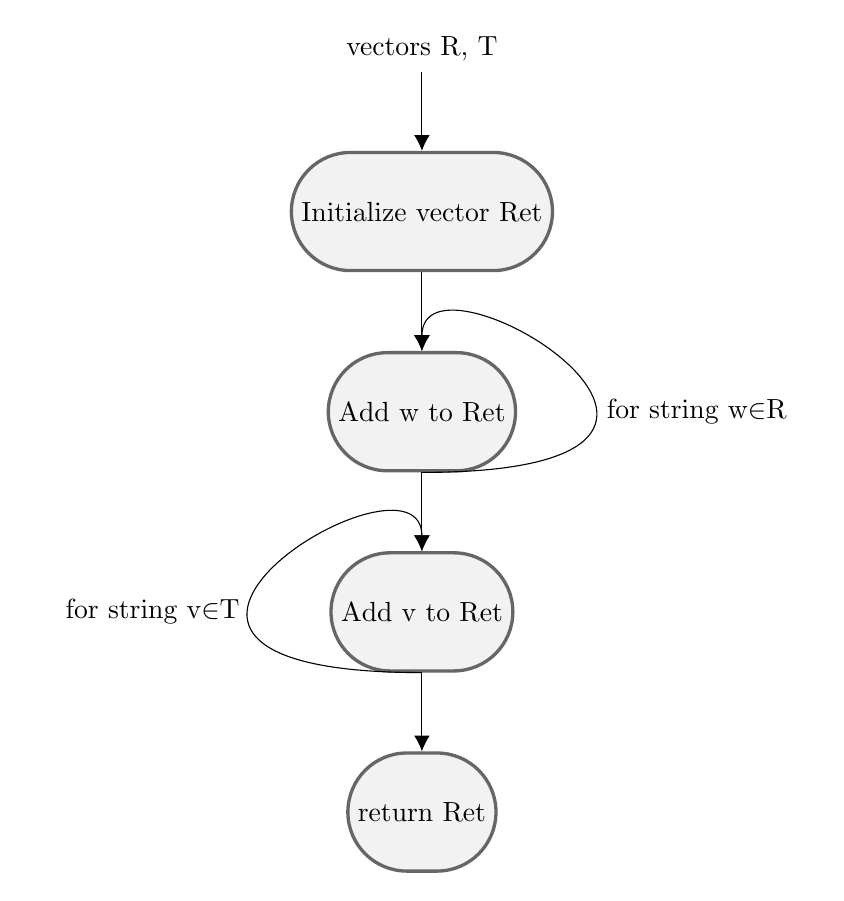
\begin{tikzpicture}[node/.style={rounded rectangle, draw=black!60, fill=black!5, very thick, minimum size=15mm}, bignode/.style={rounded rectangle, draw=black!60, fill=black!5, very thick, minimum size=20mm}, emptynode/.style={draw=none, fill=none, very thick, minimum size=1mm}]
    
    %Nodes
    \node[emptynode](inputs){vectors R, T};
    \node[node](initialize)[below=of inputs]{Initialize vector Ret};
    \node[node](add_r)[below=of initialize]{Add w to Ret};
    \node[node](add_t)[below=of add_r]{Add v to Ret};
    \node[node](return)[below=of add_t]{return Ret};
    \node[emptynode](rtext)[right=of add_r]{for string w$\in$R};
    \node[emptynode](ttext)[left=of add_t]{for string v$\in$T};
    
    %Lines
    \draw[->] (inputs.south) -- (initialize.north);
    \draw[->] (initialize.south) -- (add_r.north);
    \draw[->] (add_r.south) -- (add_t.north);
    \draw[->] (add_t.south) -- (return.north);
    \draw[->] (add_r.south) .. controls +(right:5 cm) and +(up:1.5 cm) .. (add_r.north);
    \draw[->] (add_t.south) .. controls +(left:5 cm) and +(up:1.5 cm) .. (add_t.north);
    
    \end{tikzpicture}
    \caption{Join Function}
    \label{fig:join graph}
\end{figure}

\begin{figure}[h]
    \centering
    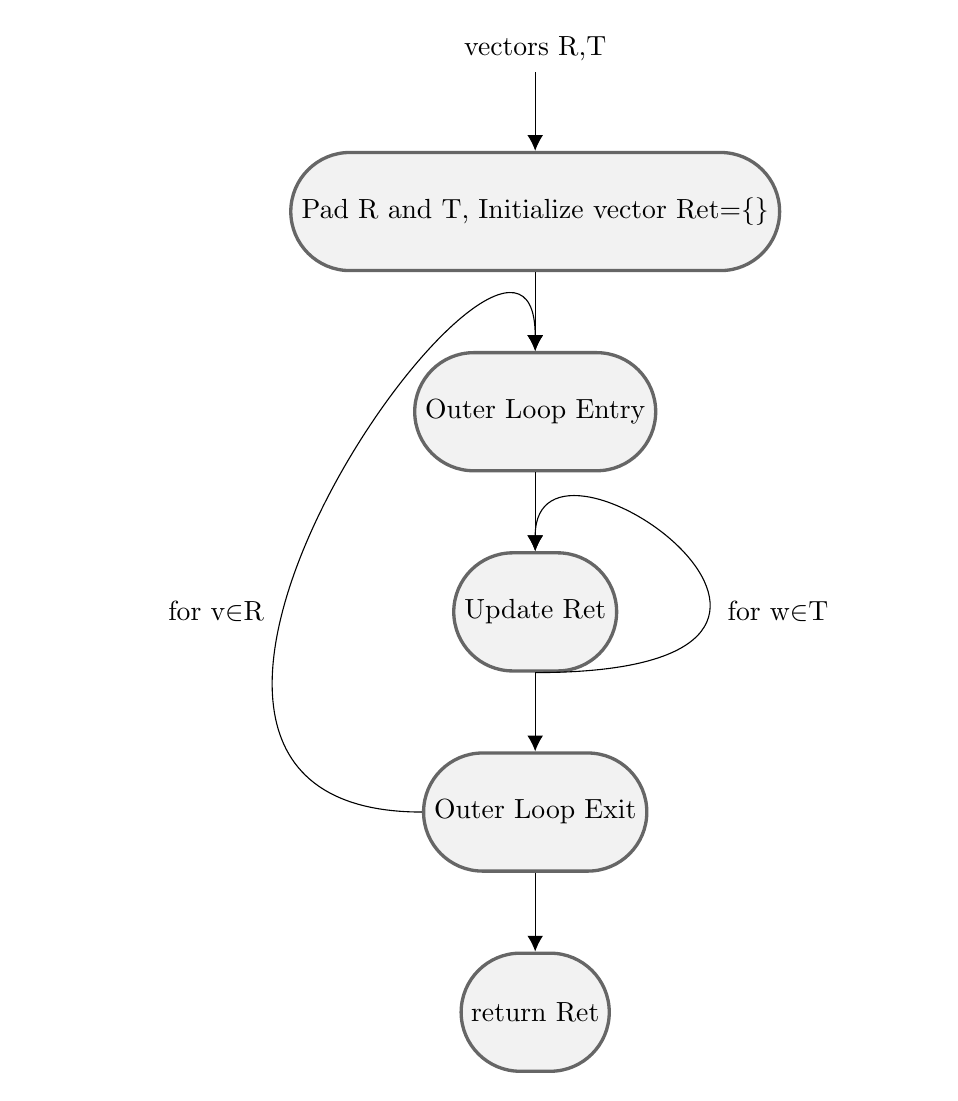
\begin{tikzpicture}[node/.style={rounded rectangle, draw=black!60, fill=black!5, very thick, minimum size=15mm}, bignode/.style={rounded rectangle, draw=black!60, fill=black!5, very thick, minimum size=20mm}, emptynode/.style={draw=none, fill=none, very thick, minimum size=1mm}]
    
    %Nodes
    \node[emptynode](inputs){vectors R,T};
    \node[node](initialize)[below=of inputs]{Pad R and T, Initialize vector Ret=\{\}};
    \node[node](outer_loop)[below=of initialize]{Outer Loop Entry};
    \node[node](inner_loop)[below=of outer_loop]{Update Ret};
    \node[node](outer_exit)[below=of inner_loop]{Outer Loop Exit};
    \node[node](return)[below=of outer_exit]{return Ret};
    \node[emptynode](inner_text)[right=1.25cm of inner_loop]{for w$\in$T};
    \node[emptynode](outer_text)[left=2.25 cm of inner_loop]{for v$\in$R};
    
    %Lines
    \draw[->] (inputs.south) -- (initialize.north);
    \draw[->] (initialize.south) -- (outer_loop.north);
    \draw[->] (outer_loop.south) -- (inner_loop.north);
    \draw[->] (inner_loop.south) -- (outer_exit.north);
    \draw[->] (outer_exit.south) -- (return.north);
    \draw[->] (inner_loop.south) .. controls +(right:5 cm) and +(up:2cm) .. (inner_loop.north);
    \draw[->] (outer_exit.west) .. controls +(left:5 cm) and +(up:3 cm) .. (outer_loop.north);
    
    \end{tikzpicture}
    \caption{Set\_Intersect Function}
    \label{fig:set_intersect graph}
\end{figure}

\begin{figure}[h]
    \centering
    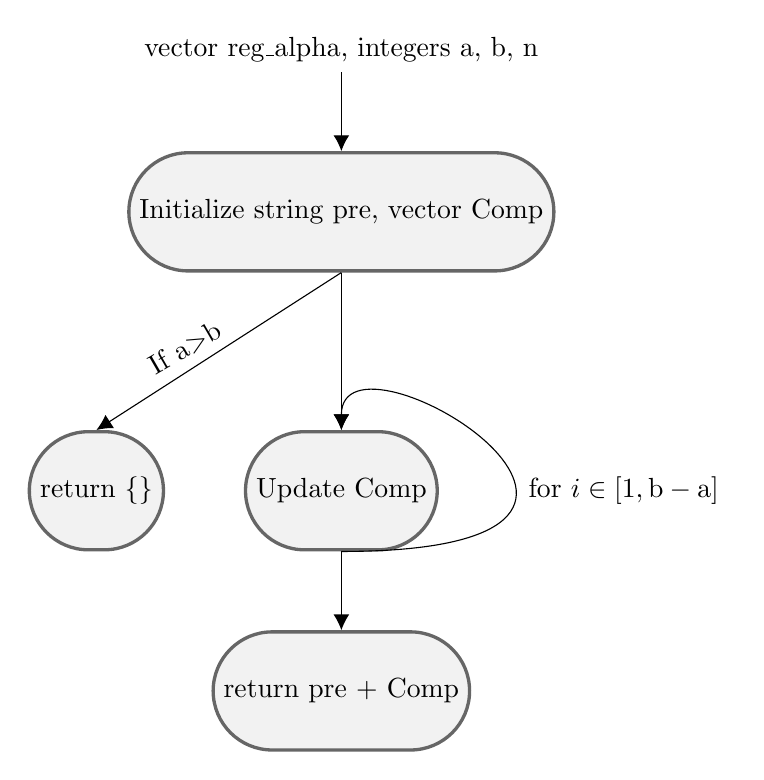
\begin{tikzpicture}[node/.style={rounded rectangle, draw=black!60, fill=black!5, very thick, minimum size=15mm}, bignode/.style={rounded rectangle, draw=black!60, fill=black!5, very thick, minimum size=20mm}, emptynode/.style={draw=none, fill=none, very thick, minimum size=1mm}]
    
    %Nodes
    \node[emptynode](inputs){vector reg\_alpha, integers a, b, n};
    \node[node](initialize)[below=of inputs]{Initialize string pre, vector Comp};
    \node[node](loop)[below=2cm of initialize]{Update Comp};
    \node[node](empty)[left=of loop]{return \{\}};
    \node[node](return)[below=of loop]{return pre + Comp};
    \node[emptynode](loop_text)[right= of loop]{for $i \in [1, \text{b}-\text{a}]$};
    \node[emptynode](placeholder)[below=0.5cm of initialize]{};
    \node[emptynode](empty_text)[rotate=30, left=1.3cm of placeholder]{If a$>$b};
    
    %Lines
    \draw[->] (inputs.south) -- (initialize.north);
    \draw[->] (initialize.south) -- (empty.north);
    \draw[->] (initialize.south) -- (loop.north);
    \draw[->] (loop.south) -- (return.north);
    \draw[->] (loop.south) .. controls +(right:5 cm) and +(up:1.5 cm) .. (loop.north);
    
    \end{tikzpicture}
    
    \caption{Reg\_F Function}
    \label{fig:reg_f graph}
\end{figure}

\begin{figure}[h]
    \centering
    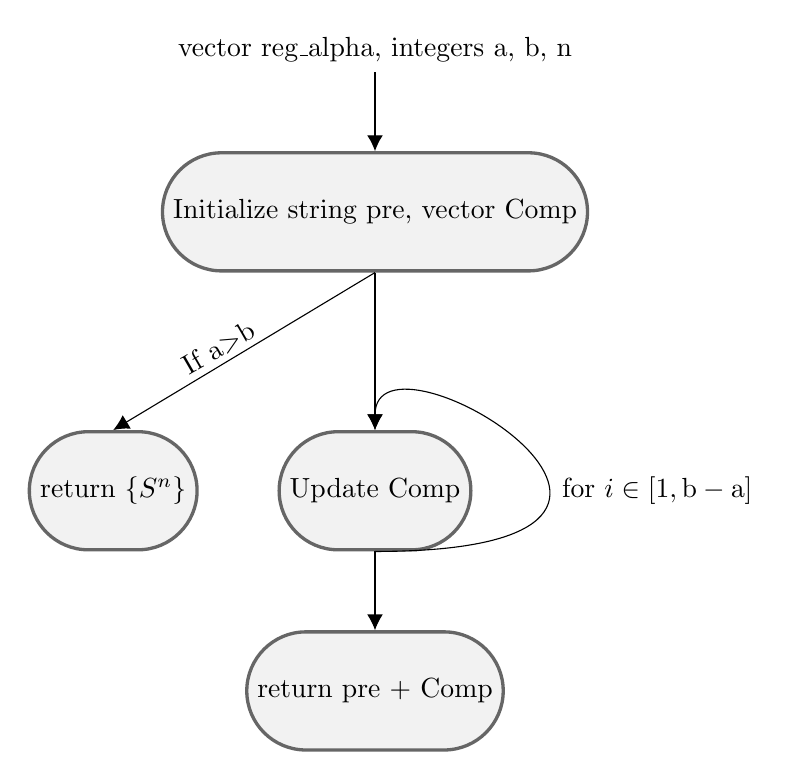
\begin{tikzpicture}[node/.style={rounded rectangle, draw=black!60, fill=black!5, very thick, minimum size=15mm}, bignode/.style={rounded rectangle, draw=black!60, fill=black!5, very thick, minimum size=20mm}, emptynode/.style={draw=none, fill=none, very thick, minimum size=1mm}]
    
    %Nodes
    \node[emptynode](inputs){vector reg\_alpha, integers a, b, n};
    \node[node](initialize)[below=of inputs]{Initialize string pre, vector Comp};
    \node[node](loop)[below=2cm of initialize]{Update Comp};
    \node[node](empty)[left=of loop]{return \{$S^n$\}};
    \node[node](return)[below=of loop]{return pre + Comp};
    \node[emptynode](loop_text)[right= of loop]{for $i \in [1, \text{b}-\text{a}]$};
    \node[emptynode](placeholder)[below=0.5cm of initialize]{};
    \node[emptynode](empty_text)[rotate=30, left=1.3cm of placeholder]{If a$>$b};
    
    %Lines
    \draw[->] (inputs.south) -- (initialize.north);
    \draw[->] (initialize.south) -- (empty.north);
    \draw[->] (initialize.south) -- (loop.north);
    \draw[->] (loop.south) -- (return.north);
    \draw[->] (loop.south) .. controls +(right:5 cm) and +(up:1.5 cm) .. (loop.north);
    
    \end{tikzpicture}
    
    \caption{Reg\_G Function}
    \label{fig:reg_g graph}
\end{figure}

\begin{figure}[h]
    \centering
    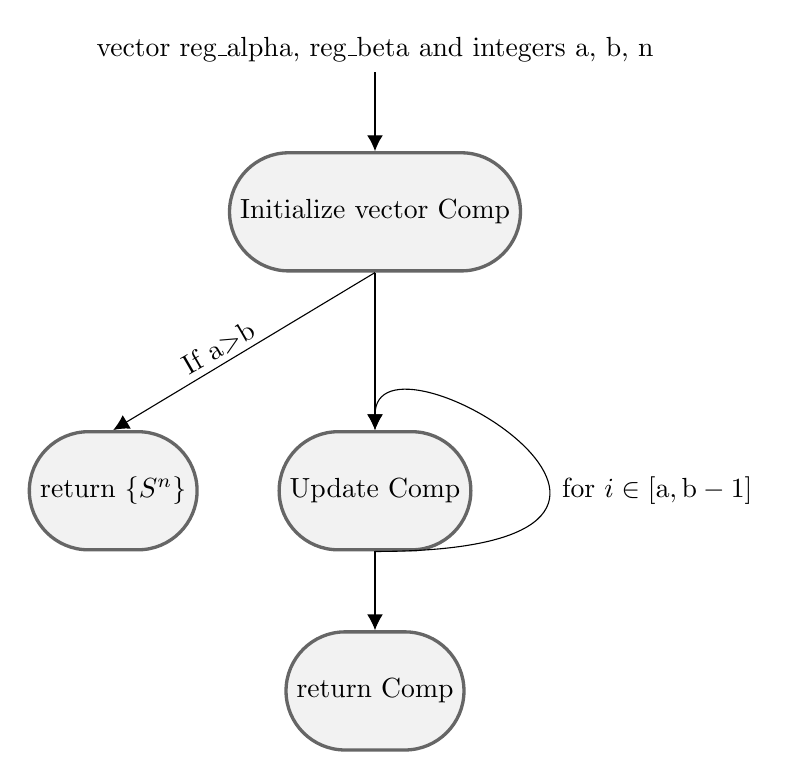
\begin{tikzpicture}[node/.style={rounded rectangle, draw=black!60, fill=black!5, very thick, minimum size=15mm}, bignode/.style={rounded rectangle, draw=black!60, fill=black!5, very thick, minimum size=20mm}, emptynode/.style={draw=none, fill=none, very thick, minimum size=1mm}]
    
    %Nodes
    \node[emptynode](inputs){vector reg\_alpha, reg\_beta and integers a, b, n};
    \node[node](initialize)[below=of inputs]{Initialize vector Comp};
    \node[node](loop)[below=2cm of initialize]{Update Comp};
    \node[node](empty)[left=of loop]{return \{$S^n$\}};
    \node[node](return)[below=of loop]{return Comp};
    \node[emptynode](loop_text)[right= of loop]{for $i \in [\text{a}, \text{b}-1]$};
    \node[emptynode](placeholder)[below=0.5cm of initialize]{};
    \node[emptynode](empty_text)[rotate=30, left=1.3cm of placeholder]{If a$>$b};
    
    %Lines
    \draw[->] (inputs.south) -- (initialize.north);
    \draw[->] (initialize.south) -- (empty.north);
    \draw[->] (initialize.south) -- (loop.north);
    \draw[->] (loop.south) -- (return.north);
    \draw[->] (loop.south) .. controls +(right:5 cm) and +(up:1.5 cm) .. (loop.north);
    
    \end{tikzpicture}
    
    \caption{Reg\_R Function}
    \label{fig:reg_r graph}
\end{figure}

\begin{figure}[h]
    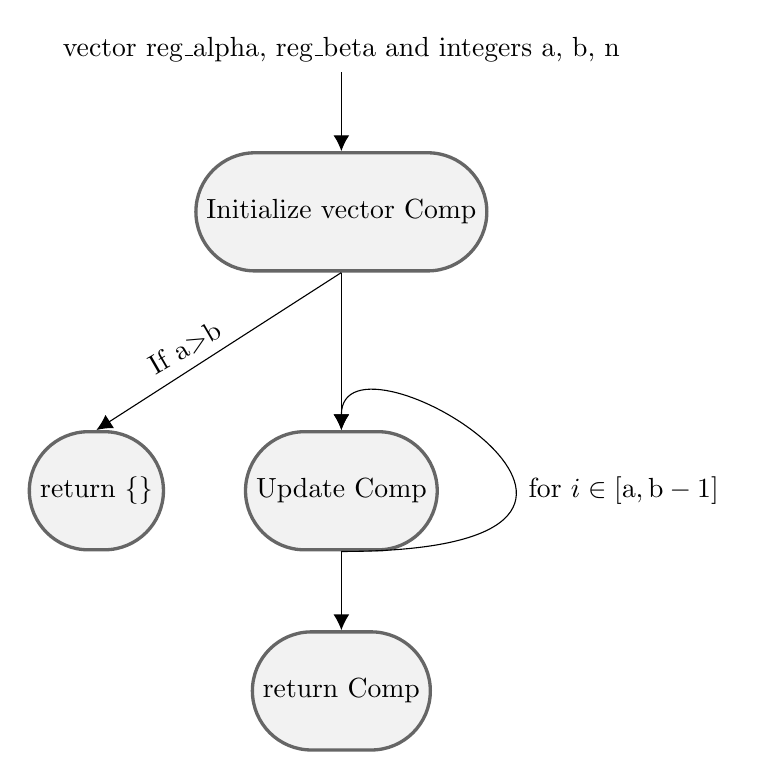
\begin{tikzpicture}[node/.style={rounded rectangle, draw=black!60, fill=black!5, very thick, minimum size=15mm}, bignode/.style={rounded rectangle, draw=black!60, fill=black!5, very thick, minimum size=20mm}, emptynode/.style={draw=none, fill=none, very thick, minimum size=1mm}]
    
    %Nodes
    \node[emptynode](inputs){vector reg\_alpha, reg\_beta and integers a, b, n};
    \node[node](initialize)[below=of inputs]{Initialize vector Comp};
    \node[node](loop)[below=2cm of initialize]{Update Comp};
    \node[node](empty)[left=of loop]{return \{\}};
    \node[node](return)[below=of loop]{return Comp};
    \node[emptynode](loop_text)[right= of loop]{for $i \in [\text{a}, \text{b}-1]$};
    \node[emptynode](placeholder)[below=0.5cm of initialize]{};
    \node[emptynode](empty_text)[rotate=30, left=1.3cm of placeholder]{If a$>$b};
    
    %Lines
    \draw[->] (inputs.south) -- (initialize.north);
    \draw[->] (initialize.south) -- (empty.north);
    \draw[->] (initialize.south) -- (loop.north);
    \draw[->] (loop.south) -- (return.north);
    \draw[->] (loop.south) .. controls +(right:5 cm) and +(up:1.5 cm) .. (loop.north);
    
    \end{tikzpicture}
    
    \caption{Reg\_U Function}
    \label{fig:reg_u graph}
\end{figure}

\begin{landscape}
\begin{figure}[h]
    \centering
    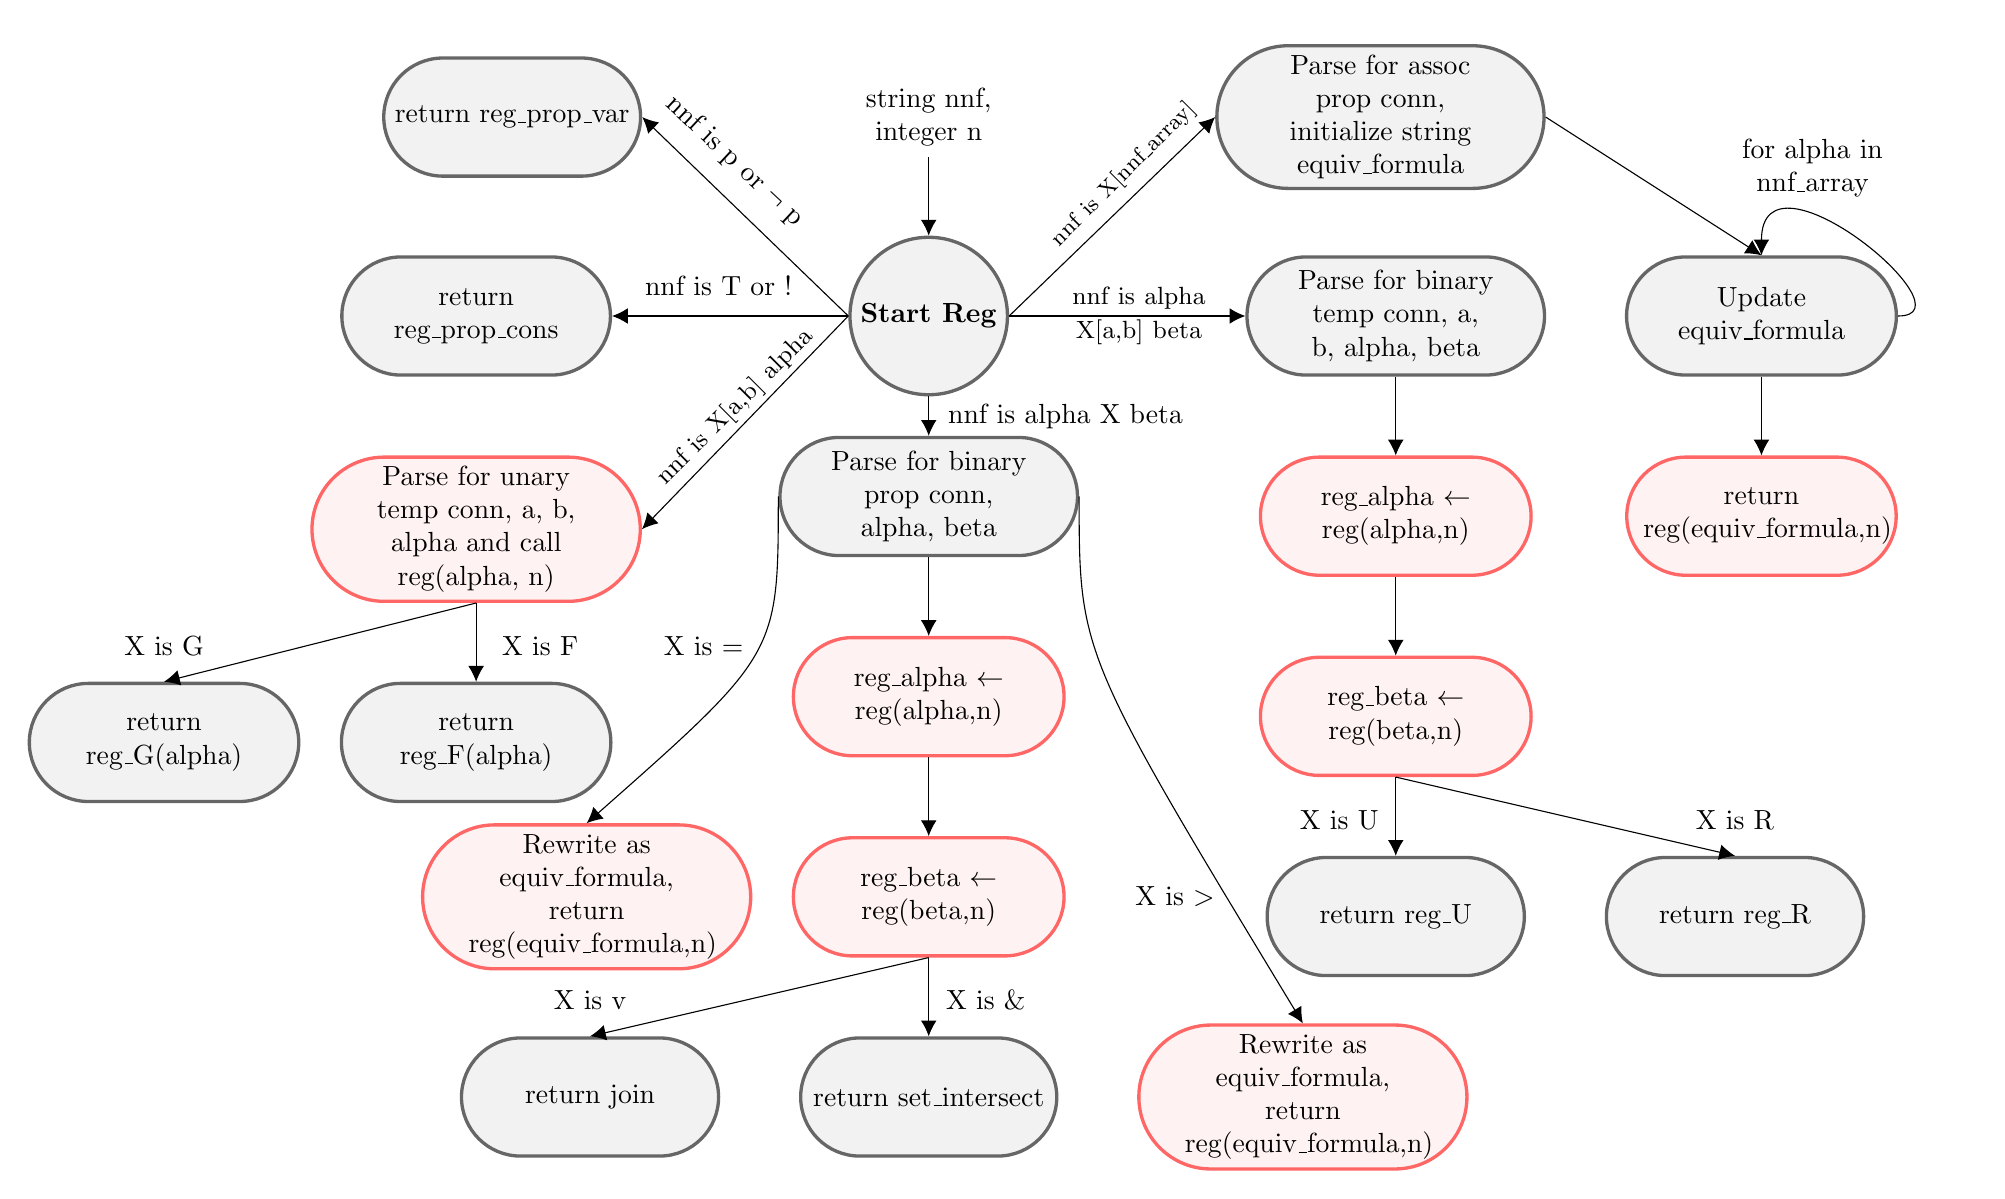
\begin{tikzpicture}[node/.style={rounded rectangle, draw=black!60, fill=black!5, text width=3cm,text centered, very thick, minimum size=15mm}, bignode/.style={rounded rectangle, draw=black!60, fill=black!5, very thick, minimum size=20mm}, emptynode/.style={draw=none, fill=none,text width=3cm,text centered, very thick, minimum size=1mm}, rednode/.style={rounded rectangle, draw=red!60, fill=red!5, text width=3cm,text centered, very thick, minimum size=15mm}]
    
    %Nodes
    \node[emptynode](inputs){string nnf, integer n};
    \node[bignode](start)[below=of inputs]{\textbf{Start Reg}};
    
    \node[node](prop_var)[left=2cm of inputs]{return reg\_prop\_var};
    
    \node[node](prop_cons)[left=3cm of start]{return reg\_prop\_cons};
    
    \node[rednode](parse_unary)[below=1cm of prop_cons]{Parse for unary temp conn, a, b, alpha and call reg(alpha, n)};
    \node[node](reg_f)[below=1cm of parse_unary]{return reg\_F(alpha)};
    \node[node](reg_g)[left=0.5cm of reg_f]{return reg\_G(alpha)};
    
    \node[node](parse_binary_prop)[below=0.5cm of start]{Parse for binary prop conn, alpha, beta};
    \node[rednode](prop_alpha)[below=of parse_binary_prop]{reg\_alpha $\leftarrow$ reg(alpha,n)};
    \node[rednode](prop_beta)[below=of prop_alpha]{reg\_beta $\leftarrow$ reg(beta,n)};
    \node[rednode](equals)[left=0.5cm of prop_beta]{Rewrite as equiv\_formula, return reg(equiv\_formula,n)};
    \node[node](set_intersect)[below=of prop_beta]{return set\_intersect};
    \node[node](join)[left=of set_intersect]{return join};
    \node[rednode](implies)[right=of set_intersect]{Rewrite as equiv\_formula, return reg(equiv\_formula,n)};
    
    \node[node](parse_binary_temp)[right=3cm of start]{Parse for binary temp conn, a, b, alpha, beta};
    \node[rednode](temp_alpha)[below=of parse_binary_temp]{reg\_alpha $\leftarrow$ reg(alpha,n)};
    \node[rednode](temp_beta)[below=of temp_alpha]{reg\_beta $\leftarrow$ reg(beta,n)};
    \node[node](until)[below=of temp_beta]{return reg\_U};
    \node[node](release)[right=of until]{return reg\_R};
    
    \node[node](parse_assoc)[right=2cm of inputs]{Parse for assoc prop conn, initialize string equiv\_formula};
    \node[node](rewrite_assoc)[right=of parse_binary_temp]{Update equiv\_formula};
    \node[rednode](assoc_return)[below=of rewrite_assoc]{return reg(equiv\_formula,n)};
    
    \node[emptynode](prop_cons_text)[left=0.01cm of start]{nnf is T or !$$~$$};
    \node[emptynode](prop_var_text)[rotate=-43, above=1.1cm of prop_cons_text]{nnf is p or $\neg$ p};
    
    \node[emptynode](unary_text)[rotate=45, below=0.3cm of prop_cons_text]{\small{nnf is X[a,b] alpha}};
    \node[emptynode](reg_g_text)[above=0.2cm of reg_g]{X is G};
    \node[emptynode](reg_f_text)[right=1.5cm of reg_g_text]{X is F};
    
    \node[emptynode](binary_temp_text)[right=0.01cm of start]{\small{nnf is alpha X[a,b] beta}};
    \node[emptynode](release_text)[above=0.2cm of release]{X is R};
    \node[emptynode](until_text)[left=1.75cm of release_text]{X is U};
    
    \node[emptynode](assoc_text)[rotate=45, above=1.1cm of binary_temp_text]{\footnotesize{nnf is X[nnf\_array]}};
    \node[emptynode](loop_text)[right=1.75cm of parse_assoc]{$$~$$for alpha in nnf\_array};
    
    \node[emptynode](binary_prop_text)[right=1.4cm of unary_text]{$$~$$$$~$$$$~$$nnf is alpha X beta};
    \node[emptynode](join_text)[above=0.2cm of join]{X is v};
    \node[emptynode](intersect_text)[right=1.75cm of join_text]{X is \&};
    \node[emptynode](implies_text)[right=-0.25cm of prop_beta]{X is $>$};
    \node[emptynode](equals_text)[right=-1.2cm of reg_f_text]{X is =};
    
    %Lines
    \draw[->] (inputs.south) -- (start.north);
    \draw[->] (start.west) -- (prop_var.east);
    \draw[->] (start.west) -- (prop_cons.east);
    \draw[->] (start.west) -- (parse_unary.east);
    \draw[->] (parse_unary.south) -- (reg_g.north);
    \draw[->] (parse_unary.south) -- (reg_f.north);
    \draw[->] (start.south) -- (parse_binary_prop.north);
    \draw[->] (parse_binary_prop.south) -- (prop_alpha.north);
    \draw[->] (prop_alpha.south) -- (prop_beta.north);
    \draw[->] (prop_beta.south) -- (set_intersect.north);
    \draw[->] (prop_beta.south) -- (join.north);
    \draw[->] (parse_binary_prop.east) .. controls +(down:2cm) .. (implies.north);
    \draw[->] (parse_binary_prop.west) .. controls +(down:2cm) .. (equals.north);
    \draw[->] (start.east) -- (parse_binary_temp.west);
    \draw[->] (parse_binary_temp.south) -- (temp_alpha.north);
    \draw[->] (temp_alpha.south) -- (temp_beta.north);
    \draw[->] (temp_beta.south) -- (until.north);
    \draw[->] (temp_beta.south) -- (release.north);
    \draw[->] (start.east) -- (parse_assoc.west);
    \draw[->] (parse_assoc.east) -- (rewrite_assoc.north);
    \draw[->] (rewrite_assoc.south) -- (assoc_return.north);
    \draw[->] (rewrite_assoc.east) .. controls +(right:1 cm) and +(up:1.5 cm) .. (rewrite_assoc.north);
    
    \end{tikzpicture}
    \caption{Control Flow}
    \label{fig:big boy}
\end{figure}
\end{landscape}

\end{document}